\chapter{Validation and Results Evaluation}%
\label{chapter:validation-and-results-evaluation}

\begin{introduction}
This chapter presents the validation process and evaluates the performance and effectiveness of the implemented solution. Through a series of defined test scenarios and experiments, quantitative and qualitative results are gathered and analyzed. These findings are then critically assessed against the initial research objectives and compared with existing approaches discussed in the state of the art.
\end{introduction}

\section{Methodology}

To assess the feasibility, functionality, and effectiveness of the proposed solution, a series of tests were conducted within the simulated environment described in the \ref{chapter:development-and-implementation} chapter. The overall validation approach was simulation-based testing, leveraging the orchestrated virtual machines and configured \ac{5G} components (Open5GS, UERANSIM) and local network services (\texttt{hostapd}, \texttt{dnsmasq}, and the custom \texttt{interceptor} application).

The validation focused on several key aspects of the system:

\subsection{Overall Validation Approach}

\begin{itemize}
    \item \textbf{Simulation-Based Testing:} All validation activities were performed within the virtualized environment created using Vagrant, Open5GS, UERANSIM, FreeRADIUS, and the custom \texttt{interceptor} application. This allowed for controlled and repeatable testing of the end-to-end solution.

    \item \textbf{Focus on Functional Correctness and Integration:} The primary goal was to verify that the proposed mechanisms for authentication, proxy identity creation (per-device \ac{PDU} session), traffic mapping, and lifecycle management operate as designed.

    \item \textbf{Qualitative Security Assessment:} While not a formal security audit, the validation included observing whether the implemented security measures (\ac{EAP-TLS}, traffic separation) were functioning as intended.
\end{itemize}

\subsection{\acs{KPI}s and Metrics for Evaluation}

The evaluation of the framework centered on the following indicators and metrics, primarily assessed through functional testing and observation of system logs and behavior:

\begin{enumerate}
    \item{
        \textbf{Functional Correctness:}
        \begin{itemize}
            \item {
                \textbf{\ac{NAUN3} Device Authentication Success:}
                \begin{itemize}
                    \item \textbf{Metric:} Successful completion of the EAP-TLS authentication process for an NAUN3 device with the FreeRADIUS server, relayed by the 5G-RG (hostapd and interceptor).

                    \item \textbf{Verification:} Logs from \texttt{wpa\_supplicant} (\texttt{naun3} \ac{VM}), \texttt{hostapd} (\ac{5G-RG}/\texttt{ue} \ac{VM}), FreeRADIUS (\texttt{core} \ac{VM}), and the custom \texttt{interceptor} application on the \ac{5G-RG}. 
                \end{itemize}
            }
            \item {
                \textbf{Dedicated \ac{PDU} Session Establishment:}
                \begin{itemize}
                    \item \textbf{Metric:} Successful establishment of a unique \ac{PDU} session on the \texttt{clients} \ac{DNN} by the \ac{5G-RG} for each successfully authenticated \ac{NAUN3} device.

                    \item \textbf{Verification:} Output of \texttt{nr-cli ps-list} command on the \ac{5G-RG} (\texttt{ue} \ac{VM}); logs from Open5GS \ac{SMF} and \ac{UPF} on the \texttt{core} \ac{VM}. 
                \end{itemize}
            }
            \item {
                \textbf{\ac{IP} Address Allocation:}
                \begin{itemize}
                    \item \textbf{Metric (Local):} Successful assignment of a local \ac{IP} address to the \ac{NAUN3} device by \texttt{dnsmasq} on the \ac{5G-RG} after \ac{EAP-TLS} authentication.

                    \item \textbf{Metric (\ac{5GC}):} Successful assignment of a \ac{5GC} \ac{IP} address by the \ac{5GC} (\ac{SMF}/\ac{UPF}) to the dedicated \ac{PDU} session for the \ac{NAUN3} device.

                    \item \textbf{Verification:} \texttt{ip addr} command output on the \texttt{naun3} \ac{VM}; \texttt{dnsmasq} logs on the \ac{5G-RG}; \texttt{nr-cli ps-list} output on the \ac{5G-RG}; Open5GS \ac{SMF}/\ac{UPF} logs. 
                \end{itemize}
            }
            \item {
                \textbf{End-to-End Data Plane Connectivity:}
                \begin{itemize}
                    \item \textbf{Metric:} Ability of an authenticated \ac{NAUN3} device to send and receive \ac{IP} traffic to/from an external network via its dedicated \ac{PDU} session. 

                    \item \textbf{Verification:} Ping tests and simple data transfer from the \texttt{naun3} \ac{VM} to a target beyond the \ac{UPF}; packet captures (\texttt{tcpdump}) on \ac{NAUN3} \ac{LAN} interface, \ac{5G-RG}'s \ac{PDU} session tunnel interface, and \ac{UPF} interfaces.
                \end{itemize}
            }
            \item {
                \textbf{Traffic Isolation and Mapping:}
                \begin{itemize}
                    \item \textbf{Metric:} Confirmation that traffic from a specific \ac{NAUN3} device is routed exclusively through its dedicated \ac{PDU} session and associated routing rules. 

                    \item \textbf{Verification:} Packet captures on the \ac{5G-RG}; analysis of \texttt{iptables} counters, \texttt{ip rule} and \texttt{ip route} configurations on the \ac{5G-RG} during active traffic from one or more \ac{NAUN3} devices. 
                \end{itemize}
            }
            \item {
                \textbf{Lifecycle Management Correctness:}
                \begin{itemize}
                    \item \textbf{Metric:} Successful de-authentication of an \ac{NAUN3} device and termination of its associated \ac{PDU} session upon simulated disconnection/unreachability.

                    \item \textbf{Verification:} Logs from the \texttt{interceptor} application, \texttt{hostapd}, and \texttt{dnsmasq}; \texttt{nr-cli ps-list} output showing \ac{PDU} session release; verification of removal of \texttt{iptables} rules and \texttt{dnsmasq} permissions.
                \end{itemize}
            }
        \end{itemize}
    }
    \item{
        \textbf{Security Aspects (Qualitative Observation):}
        \begin{itemize}
            \item \textbf{\ac{EAP-TLS} Authentication Integrity:} Observation of the complete \ac{EAP-TLS} handshake and successful mutual authentication through detailed logs from involved components (\texttt{wpa\_supplicant}, \texttt{hostapd}, FreeRADIUS).

            \item \texttt{Traffic Segregation:} Confirmation via network monitoring and \ac{PDU} session analysis that \texttt{backhaul} \ac{DNN} traffic (e.g., \ac{RADIUS}) remains logically separate from the \texttt{clients} \ac{DNN} traffic (\ac{NAUN3} user plane data).

            \item \textbf{\ac{NAUN3} Identity Concealment from \ac{5GC}:} Verification that the \ac{NAUN3} device's local identifiers (e.g., \ac{MAC} address) are not directly signaled to or stored by the core \ac{5GC} \acp{NF} (\ac{AMF}, \ac{SMF}, \ac{UDM}), with the \ac{5G-RG} acting as the boundary.
        \end{itemize}
    }
    \item{
        \textbf{Resource Management (Observational):}
        \begin{itemize}
            \item \textbf{\ac{PDU} Session Correlation:} The number of active \ac{PDU} sessions on the \texttt{clients} \ac{DNN} should directly correspond to the number of currently authenticated and connected \ac{NAUN3} devices, as tracked by the \texttt{interceptor} application.

            \item \textbf{Timeliness of Operations (Qualitative):} General observation of the time taken for the end-to-end process: \ac{NAUN3} device \ac{EAP-TLS} authentication, subsequent \ac{PDU} session establishment, and the teardown process upon device disconnection. Formal latency measurements were considered outside the primary scope of this functional validation.
        \end{itemize}
    }
    \item{
        \textbf{System Stability and Robustness (Qualitative):}
        \begin{itemize}
            \item \textbf{Handling Multiple Devices:} The ability of the \texttt{interceptor} application and the overall simulated system to manage sequential and concurrent connections and disconnections of multiple \ac{NAUN3} devices without instability.

            \item \textbf{Error Handling:} Observation of error logging and any recovery mechanisms within the \texttt{interceptor} application in scenarios such as a failed \ac{PDU} session establishment attempt or unexpected disconnection.
        \end{itemize}
    }
\end{enumerate}

This validation methodology aims to provide a comprehensive assessment of the implemented solution's ability to meet its design goals, focusing on correct functionality and integration within the simulated \ac{5G} environment. The subsequent sections will detail the specific test scenarios designed and the evaluation of the results obtained.

\section{Test Scenarios and Setup}

To validate the different aspects of the proposed framework, a series of distinct test scenarios, or experiments, were designed and executed. These scenarios leveraged the fully configured simulation environment detailed in the \ref{chapter:development-and-implementation}, which includes the \texttt{core} \ac{VM} (Open5GS, FreeRADIUS), \texttt{gnb} \ac{VM} (UERANSIM gNB), \texttt{ue} \ac{VM} (5G-RG with UERANSIM UE, \texttt{hostapd}, \texttt{dnsmasq}, and the custom \texttt{interceptor} application), and one or more \texttt{naun3} \acp{VM} (\ac{EAP} supplicant).

Specific tools were employed for monitoring and verification in each scenario:

\begin{itemize}
    \item \textbf{Log Analysis:} Reviewing logs from Open5GS \acp{NF}, UERANSIM components, FreeRADIUS, \texttt{hostapd}, \texttt{wpa\_supplicant}, and the custom \texttt{interceptor} application was fundamental across all tests.

    \item \textbf{Packet Capture:} \texttt{tcpdump} and \texttt{tshark} (Wireshark \ac{CLI}) were used on various interfaces (\ac{NAUN3} \ac{LAN}, \ac{5G-RG}'s \texttt{backhaul} and \texttt{clients} \ac{PDU} session interfaces \texttt{uesimtunX}, \ac{gNB} interfaces) to inspect signaling and data plane traffic.

    \item \textbf{Network Utilities:} Standard Linux utilities like \texttt{ping} (with the \texttt{-R} record route option), \texttt{ip addr}, \texttt{ip route}, \texttt{ip rule}, \texttt{iptables -L -v -n -t mangle -t nat -t filter}, and UERANSIM's \texttt{nr-cli} were used for connectivity testing and state verification.

    \item \textbf{Traffic Generation and Throughput Measurement:} \texttt{iperf3} was used for generating controlled \ac{TCP}/\ac{UDP} network traffic between \ac{NAUN3} devices and a server on the \texttt{core} \ac{VM} (simulating an N6-connected server) to test data plane throughput and routing.

    \item \textbf{Timestamping/Scripting:} Basic shell scripting was used to capture timestamps before and after key events (e.g., `wpa\_supplicant` start and `dhclient` IP acquisition) to measure onboarding delay.
\end{itemize}

\subsection{Experiment 1: Single \acs{NAUN3} Device Onboarding and Basic Connectivity}

The objective was to verify the successful \ac{EAP-TLS} authentication of a single \ac{NAUN3} device, the subsequent establishment of its dedicated \ac{PDU} session on the \texttt{clients} \aDNN, local and 5GC IP address allocation, basic end-to-end data plane connectivity with path verification, and to measure the approximate onboarding delay.

Procedure:
\begin{enumerate}
    \item Ensure all \ac{5GC} \acp{NF}, \ac{gNB}, \ac{5G-RG} (including \texttt{hostapd} and \texttt{interceptor}), and FreeRADIUS are running. Start an \texttt{iperf3} server on the \texttt{core} \ac{VM} listening on the \ac{IP} address of its \texttt{clientun0} interface (e.g., \texttt{10.46.0.1}).

    \item On the \texttt{naun3} \ac{VM}, record a timestamp (\texttt{date +\%s}). Immediately start the \texttt{wpa\_supplicant} service.

    \item Monitor the authentication process through logs on the \texttt{naun3} \ac{VM}, \texttt{ue} \ac{VM} (\texttt{hostapd}, \texttt{interceptor}), and \texttt{core} \ac{VM} (FreeRADIUS).

    \item Once \texttt{wpa\_supplicant} indicates success and \texttt{dhclient} (run subsequently or as part of the script on \texttt{naun3}) obtains a local \ac{IP}, record another timestamp. Calculate the difference to estimate onboarding delay.
    
    \item Verify \ac{PDU} session establishment for the \texttt{clients} \ac{DNN} using \textttnr{-cli ps-list} on the \texttt{ue} \ac{VM}. Note the assigned \ac{5GC} \ac{IP} address for this \ac{PDU} session.
    
    \item Verify local \ac{IP} address assignment to the \texttt{naun3} \ac{VM} via \texttt{ip addr} on the \texttt{naun3} \ac{VM}.
    
    \item Verify the application of \texttt{iptables} and \texttt{ip rule}/\texttt{ip route} rules on the \texttt{ue} \ac{VM} specific to the authenticated \ac{NAUN3} device's \ac{MAC} and \ac{PDU} session ID.
    
    \item From the \texttt{naun3} \ac{VM}, initiate \texttt{ping -R <PDU\_Session\_Gateway\_IP>} (e.g., \texttt{10.46.0.1}). Analyze the recorded route to confirm it passes through the \ac{NAUN3}'s local \ac{IP}, then its assigned \ac{5GC} \ac{PDU} session \ac{IP}, and then to the target.
    
    \item From the \texttt{naun3} \ac{VM}, run an \texttt{iperf3} client connecting to the \texttt{iperf3} server on the \texttt{core} \ac{VM}.
    
    \item Capture traffic on relevant interfaces (\texttt{naun3} \ac{LAN}, \texttt{ue} \ac{VM} \ac{LAN}, \texttt{uesimtunX} on \texttt{ue} \ac{VM}, \texttt{clientun0} on \texttt{core} \ac{VM}) to observe data flow and \ac{NAT}.
\end{enumerate}

Metrics/Verification Points:
\begin{itemize}
    \item Successful \ac{EAP-TLS} authentication (logs).
    \item Onboarding delay (timestamp difference).
    \item One new \ac{PDU} session active on \texttt{clients} \ac{DNN} for the \ac{5G-RG}, with a unique \ac{5GC} \ac{IP}.
    \item \ac{NAUN3} device receives a local \ac{IP}.
    \item Successful \texttt{ping} with recorded route showing \ac{NAT} via the \ac{PDU} session IP.
    \item Successful \texttt{iperf3} data transfer.
    \item Correct \texttt{iptables} and policy routing rules applied.
\end{itemize}

\subsection{Experiment 2: Multi-Device Connectivity, Traffic Isolation, and \acs{PDU} Session Mapping}

In this experiment the goal was to verify that when multiple \ac{NAUN3} devices connect simultaneously, each gets a unique dedicated \ac{PDU} session, their traffic is correctly mapped and isolated, and \ac{NAT} occurs via their respective \ac{PDU} session \acp{IP}.

Procedure:
\begin{enumerate}
    \item Start two (or more) \texttt{naun3} \acp{VM} (e.g., \textt{naun301}, \texttt{naun302}), each configured with a client certificates for \ac{EAP-TLS}.

    \item Allow both devices to authenticate and establish their dedicated \ac{PDU} sessions as per Experiment 1. Verify that two distinct \texttt{clients} \ac{PDU} sessions are created by the \ac{5G-RG}, each with a unique \ac{5GC} \ac{IP} address (e.g., \texttt{10.46.0.3} and \texttt{10.46.0.4}).
    
    \item On the \texttt{ue} \ac{VM}, verify that distinct sets of \texttt{iptables} and \texttt{ip rule}/\texttt{ip route} entries are created for each \ac{NAUN3} device, mapping each to its unique \ac{PDU} session ID and tunnel interface.
    
    \item From \texttt{naun301}, execute \texttt{ping -R <PDU\_Session\_Gateway\_IP>}. Note the recorded route, particularly the \ac{5GC} \ac{IP} address assigned to \texttt{naun301}'s \ac{PDU} session.
    
    \item From \texttt{naun302}, execute \texttt{ping -R <PDU\_Session\_Gateway\_IP>}. Note the recorded route, verifying it uses a \textit{different} \ac{5GC} \ac{IP} address assigned to \texttt{naun302}'s \ac{PDU} session.
    
    \item Start an \texttt{iperf3} server on the \texttt{core} \ac{VM}.
    
    \item Simultaneously (or sequentially) run \texttt{iperf3} clients from \texttt{naun301} and \texttt{naun302} to the server on the \texttt{core} \ac{VM}.
    
    \item Monitor traffic on the \texttt{ue} \ac{VM}'s \texttt{uesimtunX} interfaces and check \texttt{iptables} counters to confirm traffic from each \ac{NAUN3} device is routed through its distinct \ac{PDU} session.
    
    \item On the \texttt{core} \ac{VM} (\texttt{iperf3} server logs), verify that connections are received from the distinct \ac{5GC} \ac{IP} addresses assigned to each \ac{NAUN3}'s \ac{PDU} session.
\end{enumerate}

Metrics/Verification Points:
\begin{itemize}
    \item Each \ac{NAUN3} device establishes its own unique \ac{PDU} session on the \texttt{clients} \ac{DNN} with a distinct \ac{5GC} \ac{IP}.
    
    \item \texttt{ping -R} from each \ac{NAUN3} shows a path \textit{NATted} through its unique \ac{PDU} session \ac{IP}.
    
    \item \texttt{iperf3} server logs show connections from distinct \ac{PDU} session \acp{IP}.
    
    \item \texttt{iptables} and routing rules correctly isolate traffic per device.
\end{itemize}

\subsection{Experiment 3: Lifecycle Management (Device Disconnection and Resource Cleanup)}

In order to verify that when an \ac{NAUN3} device disconnects or becomes unreachable, its local authentication is revoked, its dedicated \ac{PDU} session is terminated, and associated network resources (\ac{IP} addresses, routing rules) are correctly cleaned up by the \texttt{interceptor} the following procedure was followed.

\begin{enumerate}
    \item Successfully onboard a single \ac{NAUN3} device as per Experiment 1. Verify its \ac{PDU} session is active and traffic flows.

    \item{ Simulate device disconnection:
        \begin{itemize}
            \item \textbf{Option A (Graceful):} Stop the \texttt{wpa\_supplicant} service on the \texttt{naun3} \ac{VM}.
            \item \textbf{Option B (Abrupt):} Power off or disconnect the network interface of the \texttt{naun3} \ac{VM}.
        \end{itemize}
    }

    \item Monitor the \texttt{interceptor} logs on the \texttt{ue} \ac{VM} for detection of device unreachability and initiation of cleanup procedures.

    \item{
        Verify the following cleanup actions occur:
        \begin{itemize}
            \item \texttt{hostapd} deauthenticates the client (logs).

            \item The \texttt{interceptor} removes the device's \ac{MAC} from \texttt{/etc/allowed-macs.conf} and restarts \texttt{dnsmasq}.

            \item The \texttt{interceptor} removes the specific \texttt{iptables} and \texttt{ip rule}/\texttt{ip route} entries for the device.

            \item The \texttt{interceptor} initiates a \ac{PDU} session release for the \texttt{clients} \ac{DNN} using \texttt{nr-cli}.

            \item Verify using \texttt{nr-cli ps-list} that the \ac{PDU} session is terminated.
            
            \item Verify in Open5GS \ac{SMF}/\ac{UPF} logs that the session and associated resources are released.
        \end{itemize}
    }    
\end{enumerate}

Metrics/Verification Points:
\begin{itemize}
    \item Detection of device disconnection by the \texttt{interceptor}.
    \item Successful local deauthentication.
    \item Removal of \ac{DHCP} permission.
    \item Correct removal of all associated \texttt{iptables} and routing rules.
    \item Successful \ac{PDU} session termination in UERANSIM and Open5GS.
    \item Internal state of the \texttt{interceptor} (e.g., \texttt{allowedDevices} map) reflects the device removal.
\end{itemize}

\subsection{Experiment 4: Security Aspects Observation (Qualitative)}

To qualitatively observe key security aspects of the implemented solution, such as the \ac{EAP-TLS} handshake and traffic segregation, we performed the following:

\begin{enumerate}
    \item{
        During Experiment 1 (\ac{NAUN3} Device Onboarding):
        \begin{itemize}
            \item Use \texttt{tshark} or \texttt{tcpdump} on the \texttt{ue} \ac{VM}'s \ac{LAN} interface to capture the \ac{EAPOL} and \ac{EAP-TLS} handshake.

            \item Use \texttt{tshark} or \texttt{tcpdump} on the \texttt{ue} \ac{VM}'s \texttt{backhaul} \ac{PDU} session interface and on the \texttt{core} \ac{VM}'s interface connected to the \texttt{ue} \ac{VM}'s \texttt{backhaul} to capture \ac{RADIUS} traffic.
        \end{itemize}
    }
    \item{
        During Experiment 2 (Multiple Devices):
        \begin{itemize}
            \item Observe the source and destination \acp{IP} of the \ac{RADIUS} traffic on the \texttt{backhaul} \ac{PDU} session.
            
            \item Observe the source and destination \acp{IP} of the \ac{NAUN3} user plane traffic on the respective \texttt{clients} \ac{PDU} sessions.
        \end{itemize}
    }
\end{enumerate}

Metrics/Verification Points:
\begin{itemize}
    \item Observation of a complete and successful \ac{EAP-TLS} handshake.
    \item Confirmation that \ac{RADIUS} traffic is encapsulated and transported over the \texttt{backhaul} \ac{PDU} session.
    \item Confirmation that user plane traffic for each \ac{NAUN3} device is transported over its distinct \texttt{clients} \ac{PDU} session.
    \item Review of Open5GS logs (\ac{AMF}, \ac{SMF}) to confirm that only the \ac{5G-RG}'s identity (\ac{IMSI}) is used for \ac{5GC} signaling, and \ac{NAUN3} \ac{MAC} addresses are not propagated to these core \acp{NF}.
\end{itemize}

These experiments are designed to provide a holistic view of the system's functionality, its ability to manage multiple devices correctly, handle their lifecycle, and maintain basic security and traffic segregation principles, incorporating the specific types of data you've collected.

\section{Functional Validation Results}

This section presents the results obtained from executing the test scenarios described previously, demonstrating the functional correctness of the proposed authentication and identity management mechanisms. The evidence is drawn from system logs, network interface states, routing table configurations, and packet captures.

\subsection{\acs{NAUN3} Device Authentication and Onboarding:}
The primary test involved onboarding \ac{NAUN3} devices (\texttt{naun301}, \texttt{naun302}) one after another.

\begin{itemize}
    \item \textbf{EAP-TLS Authentication:} Logs from \texttt{wpa\_supplicant} on each \ac{NAUN3} device (see Listing \ref{lst:wpa_supplicant_eap_success}) confirmed the initiation and successful completion of the \ac{EAP-TLS} handshake ("\texttt{CTRL-EVENT-EAP-SUCCESS EAP authentication completed successfully}"). Correspondingly, the \texttt{hostapd} log on the 5G-RG (\texttt{ue} \ac{VM}) showed the \ac{EAP} exchange, including the relay of messages to the \ac{RADIUS} server and the reception of Access-Accept (see Listing \ref{lst:hostapd_naun301_eap_success}). The \texttt{interceptor} (see Figure \ref{fig:interceptor_eap_success}) captured the \texttt{CTRL-EVENT-EAP-SUCCESS} from \texttt{hostapd}, indicating its awareness of the successful local authentication.

    \begin{lstlisting}[caption=wpa\_supplicant successful authentication,label={lst:wpa_supplicant_eap_success}]
(...)
584| 1748702590.706948: enp0s8: CTRL-EVENT-EAP-SUCCESS EAP authentication completed successfully
585| 1748702590.706998: EAPOL: IEEE 802.1X for plaintext connection; no EAPOL-Key frames required
586| 1748702590.707047: enp0s8: WPA: EAPOL processing complete
587| 1748702590.707096: enp0s8: Cancelling authentication timeout
586| 1748702590.707147: enp0s8: State: ASSOCIATED -> COMPLETED
586| 1748702590.707201: enp0s8: CTRL-EVENT-CONNECTED - Connection to 01:80:c2:00:00:03 completed [id=0 id_str=]
(...)
    \end{lstlisting}

    \begin{lstlisting}[caption=\texttt{hostapd} successful authentication,label={lst:hostapd_naun301_eap_success}]
(...)
802| 1748702590.717640: EAP: EAP entering state SUCCESS2
803| 1748702590.717722: enp0s9: CTRL-EVENT-EAP-SUCCESS2 08:00:27:b4:18:a9
804| 1748702590.717775: CTRL_IFACE monitor send /tmp/interceptor_7025.sock\x00
805| 1748702590.717923: IEEE 802.1X: 08:00:27:b4:18:a9 BE_AUTH entering state SUCCESS
806| 1748702590.718200: 1748702590.718200: enp0s9: STA 08:00:27:b4:18:a9 IEEE 802.1X: Sending EAP Packet (identifier 224)
807| 1748702590.718452: IEEE 802.1X: 08:00:27:b4:18:a9 AUTH_PAE entering state AUTHENTICATED
808| 1748702590.718565: enp0s9: AP-STA-CONNECTED 08:00:27:b4:18:a9
(...)
    \end{lstlisting}

    \item{
        \textbf{Dedicated \ac{PDU} Session Establishment:} Following each successful \ac{EAP-TLS} authentication, the \texttt{interceptor} log shows the initiation of a new \ac{PDU} session request for the \texttt{clients} \ac{DNN} (see Figure \ref{fig:interceptor_eap_success}). The UERANSIM tool \texttt{nr-cli ps-list} on the \ac{5G-RG}, corroborates this (see Listing \ref{fig:ue_pdu_sessions}):
        \begin{itemize}
            \item Initially (14:43:09 \ac{UTC}), only \texttt{PDU Session1} (\ac{DNN}: \texttt{backhaul}, \ac{IP}: \texttt{10.45.0.2}) is active.
            
            \item After \texttt{naun301} (\ac{MAC} \texttt{08:00:27:b4:18:a9}) authenticates (around 14:43:10 \ac{UTC} in \texttt{interceptor} log), \texttt{PDU Session2} (\ac{DNN}: \texttt{clients}, \ac{IP}: \texttt{10.46.0.2}) becomes active by 14:43:30 \ac{UTC}.

            \item After \texttt{naun302} (\ac{MAC} \texttt{08:00:27:51:7f:ef}) authenticates (around 14:44:08 \ac{UTC} in \texttt{interceptor} log), \texttt{PDU Session3} (\ac{DNN}: \texttt{clients}, \ac{IP}: \texttt{10.46.0.3}) becomes active by 14:44:30 \ac{UTC}.
        \end{itemize}

        \begin{figure}
        \centering
            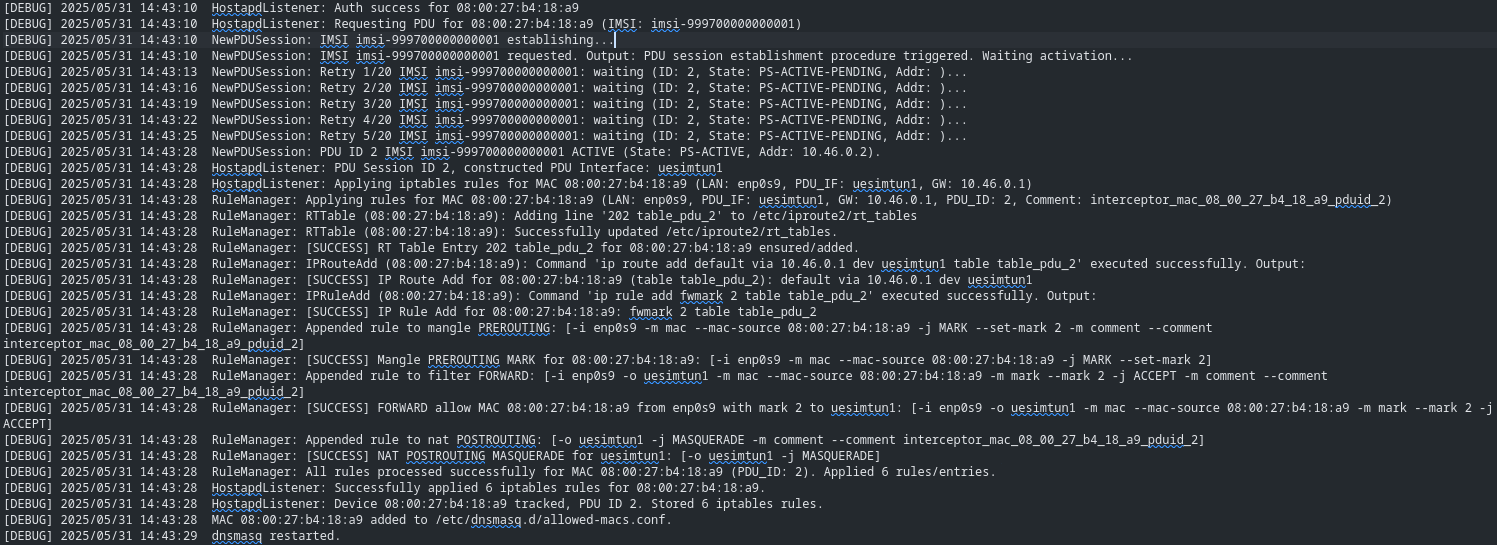
\includegraphics[width=1\linewidth]{figs/interceptor_eap_success.png}
            \caption{\texttt{interceptor} captures authentication success, requests \ac{PDU} session and applies mapping rules}
            \label{fig:interceptor_eap_success}
        \end{figure}

        \begin{figure}
            \centering
            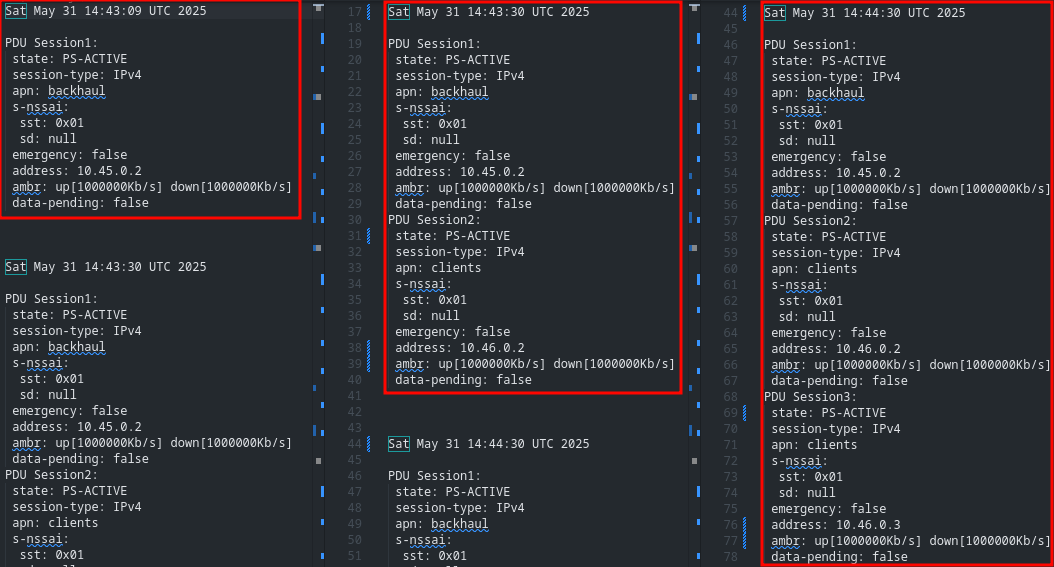
\includegraphics[width=1\linewidth]{figs/ue_pdu_sessions.png}
            \caption{\ac{PDU} Session via \texttt{nr-cli ps-list}}
            \label{fig:ue_pdu_sessions}
        \end{figure}
    }

    \item \textbf{Network Interface Creation:} The \texttt{ue} (see Figure \ref{fig:ue_pdu_sessions_nics}) log confirms the dynamic creation of network interfaces on the \ac{5G-RG} for each \texttt{clients} \ac{PDU} session. \texttt{uesimtun0} (\ac{IP} \texttt{10.45.0.2}) corresponds to the \texttt{backhaul} session. \texttt{uesimtun1} (\ac{IP} \texttt{10.46.0.2}) appears after \texttt{naun301} connects, and \texttt{uesimtun2} (\ac{IP} \texttt{10.46.0.3}) appears after \texttt{naun302} connects.

    \begin{figure}
        \centering
        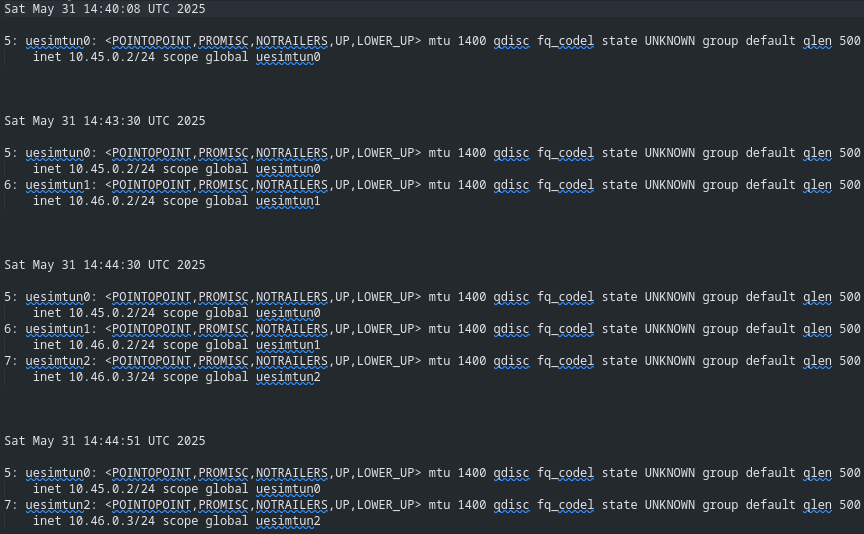
\includegraphics[width=1\linewidth]{figs/ue_pdu_sessions_nics.png}
        \caption{Network interfaces created by UERANSIM to bind to \ac{PDU} Sessions}
        \label{fig:ue_pdu_sessions_nics}
    \end{figure}

    \item \textbf{\ac{IP} Address Allocation:} The \ac{NAUN3} devices successfully obtained local \ac{IP} addresses from \texttt{dnsmasq} on the \ac{5G-RG} after authentication (see Figure \ref{fig:ping_gw}). The \ac{5GC} assigned unique \acp{IP} (\texttt{10.46.0.2}, \texttt{10.46.0.3}) to their respective \ac{PDU} sessions, as confirmed by Figures \ref{fig:ue_pdu_sessions} and \ref{fig:ue_pdu_sessions_nics}.

    \begin{figure}
        \centering
        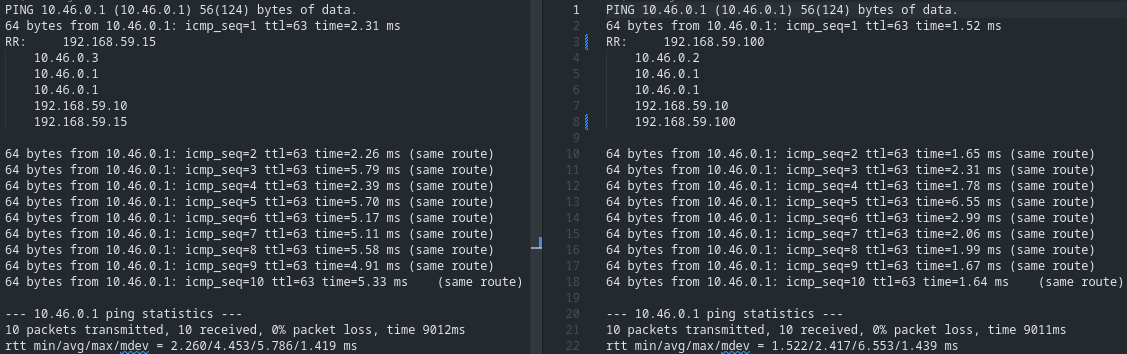
\includegraphics[width=1\linewidth]{figs/ping_gw.png}
        \caption{Pings from \texttt{naun301} and \texttt{naun302} to the \ac{5GC} gateway}
        \label{fig:ping_gw}
    \end{figure}
\end{itemize}

\subsection{End-to-End Connectivity and Path Verification}

Ping tests with the record route option (\texttt{-R}) were conducted from \texttt{naun301} and \texttt{naun302} (see Figure \ref{fig:ping_gw}) to the clients \ac{DNN} gateway \ac{IP} on the \texttt{core} \ac{VM} (\texttt{10.46.0.1}).

\begin{itemize}
    \item The recorded route when \texttt(naun301) pings the \ac{5GC} gateway is, \texttt{192.168.59.100} (\texttt{naun301} local \ac{IP}) -> \texttt{10.46.0.2} (\ac{PDU} Session 2 \ac{IP} for \texttt{naun302}) -> \texttt{10.46.0.1} (Target). This clearly demonstrates that traffic from \texttt{naun301} is \textit{NATted} using the \ac{IP} address of its dedicated \ac{PDU} session.

    \item The recorded route is \texttt{naun302} pings the \ac{5GC} gateway is, \texttt{192.168.59.15} (\texttt{naun302} local \ac{IP}) -> \texttt{10.46.0.3} (\ac{PDU} Session 3 \ac{IP} for \texttt{naun302}) -> \texttt{10.46.0.1} (Target). This confirms that \texttt{naun302}'s traffic is also \textit{NATted}, but crucially, via its own distinct \ac{PDU} session \ac{IP}.
\end{itemize}

\subsection{Traffic Isolation and Correct \acs{PDU} Session Mapping (Multiple Devices)}

\begin{figure}
    \centering
    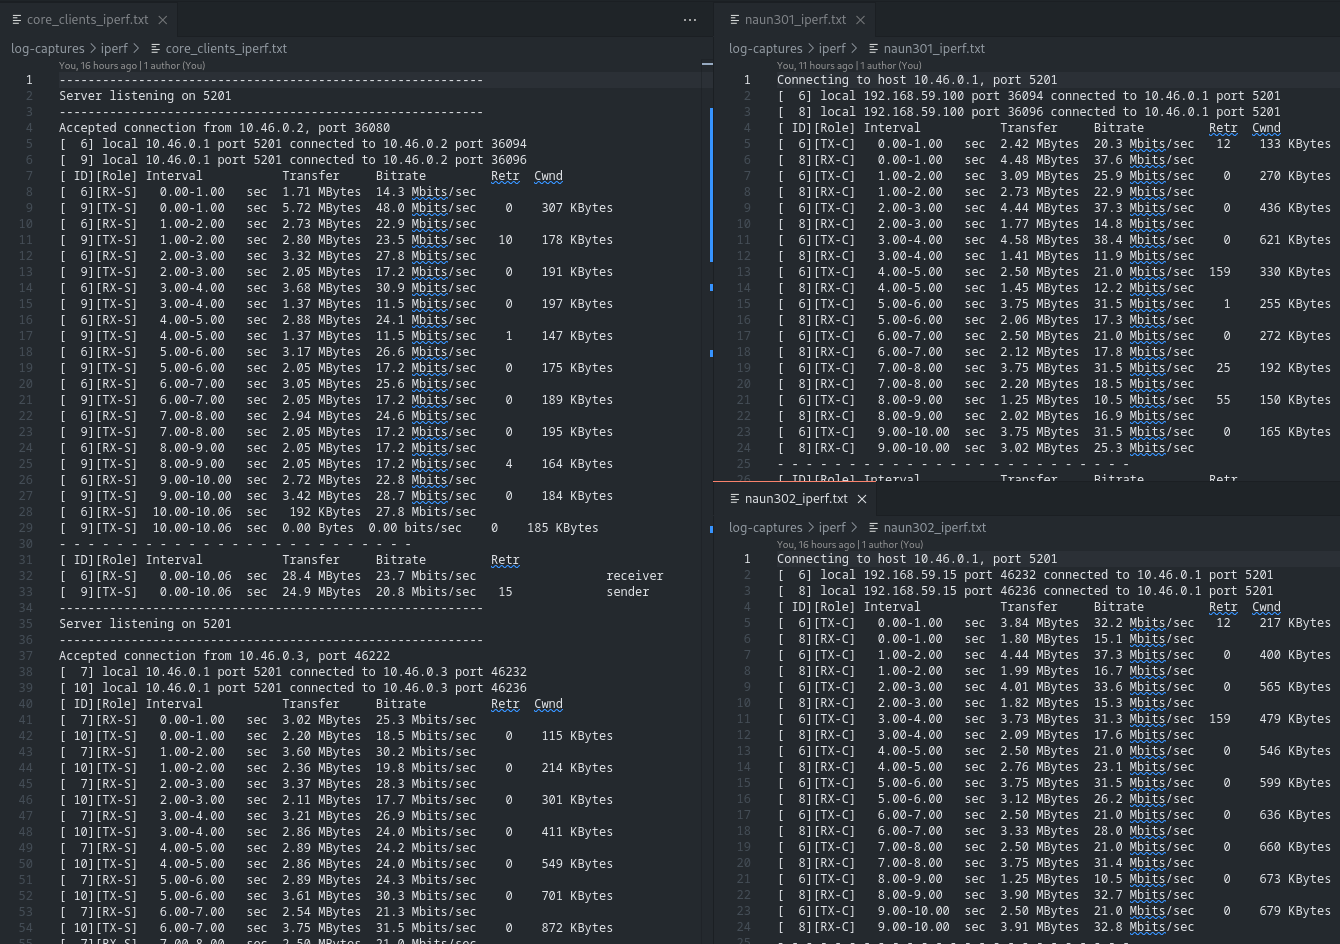
\includegraphics[width=1\linewidth]{figs/iperf_naun3_to_core.png}
    \caption{\texttt{iperf3} session between \acp{NAUN3} and \ac{5GC}}
    \label{fig:iperf_naun3_to_core}
\end{figure}

The \texttt{iperf3} tests further validated traffic isolation and mapping. As seen in the Figure \ref{fig:iperf_naun3_to_core}, it shows the \texttt{iperf3} server on \texttt{10.46.0.1} (on the left) accepting connections from two different source \acp{IP}: \texttt{10.46.0.2} and \texttt{10.46.0.3}. These correspond to the unique \ac{PDU} session \acp{IP} assigned to \texttt{naun301} and \texttt{naun302} respectively. This confirms that traffic from each \ac{NAUN3} device is correctly mapped to its dedicated \ac{PDU} session and is identifiable by this unique \ac{PDU} session \ac{IP} at the N6 network.

\begin{figure}
    \centering
    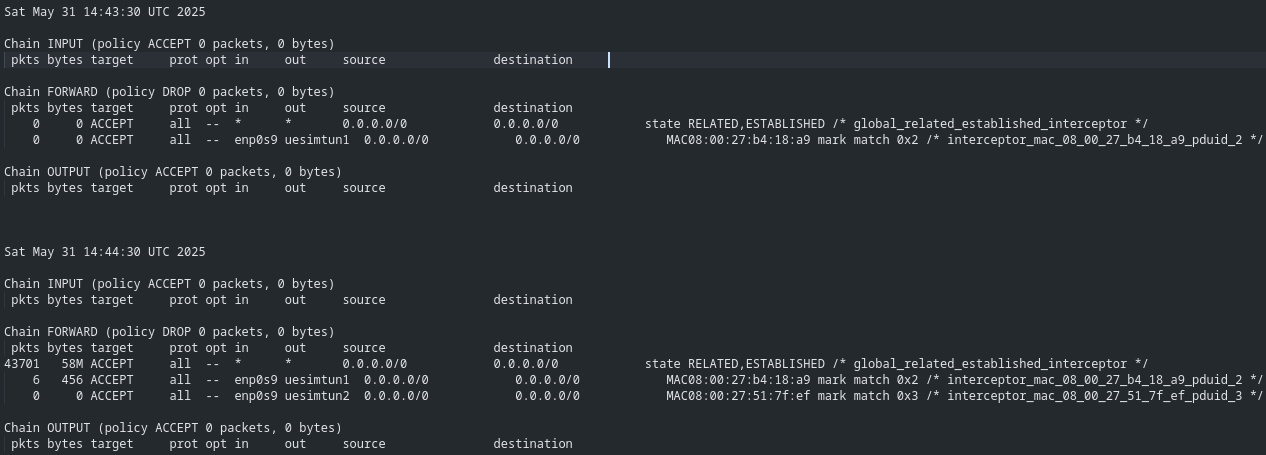
\includegraphics[width=1\linewidth]{figs/iptable_mapping_rules.png}
    \caption{\texttt{iptables} mapping rules and tables for segregating traffic}
    \label{fig:iptable_mapping_rules}
\end{figure}

Also, Figure \ref{fig:iptable_mapping_rules} shows the dynamic application of \texttt{iptables FORWARD} rules and \texttt{ip rule}/\texttt{ip route} entries. For instance, at 14:43:30 \ac{UTC} (after \texttt{naun301} connects), rules are present for \ac{MAC} \texttt{08:00:27:b4:18:a9} (\ac{naun301}) to use \ac{PDU} ID 2 (interface \texttt{uesimtun1}). By 14:44:30 \ac{UTC} (after \texttt{naun302} connects), additional rules appear for \ac{MAC} \texttt{08:00:27:51:7f:ef} (\texttt{naun302}) to use \ac{PDU} ID 3 (interface \texttt{uesimtun2}), while rules for \ac{PDU} ID 2 remain. This demonstrates the per-device rule application.

\begin{figure}
    \centering
    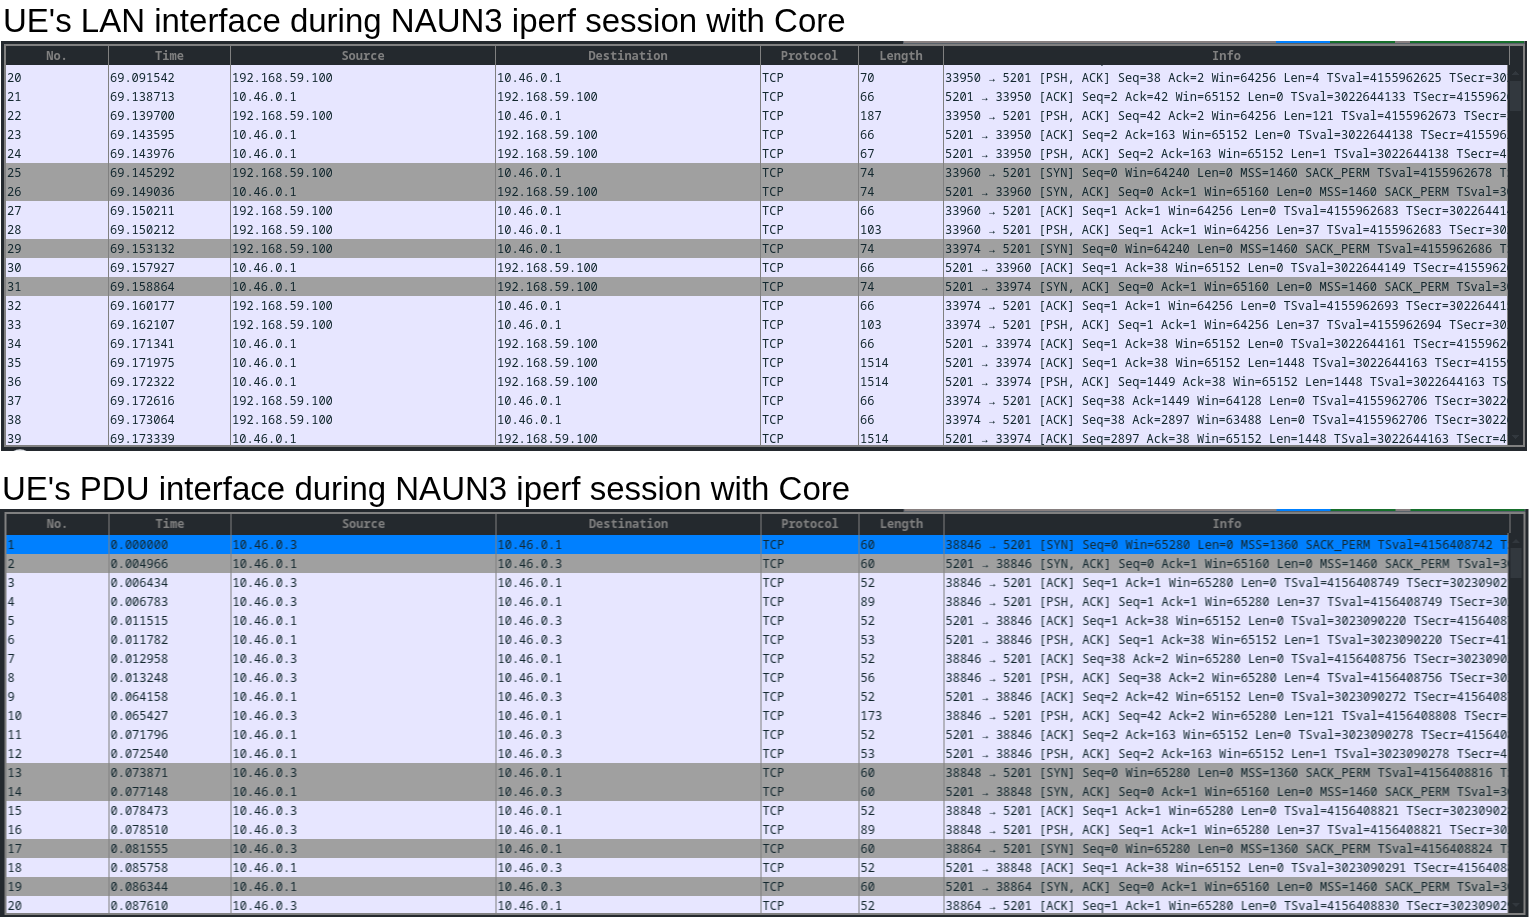
\includegraphics[width=1\linewidth]{figs/naun3_to_core_ue_view.png}
    \caption{\ac{NAUN3} to \ac{5GC} \texttt{iperf3} session, captured at the \ac{5G-RG} showing the mapping between the local address and \ac{PDU} session address}
    \label{fig:naun3_to_core_ue_view}
\end{figure}

The Wireshark capture in Figure \ref{fig:naun3_to_core_ue_view} visually confirms this: traffic on the \ac{5G-RG}'s \ac{LAN} interface shows the \ac{NAUN3}'s local \ac{IP} (e.g., \texttt{192.168.59.100}), while on the corresponding \ac{PDU} session tunnel interface (\texttt{uesimtunX}), the source \ac{IP} is the \ac{PDU} session's \ac{5GC}-assigned \ac{IP} (e.g., \texttt{10.46.0.3})

\subsection{Lifecycle Management (Device Disconnection)}

The logs demonstrate correct resource cleanup when \texttt{naun301} (associated with \ac{PDU} Session2, \ac{IP} \texttt{10.46.0.2}, interface \texttt{uesimtun1}) disconnects:

\begin{figure}
    \centering
    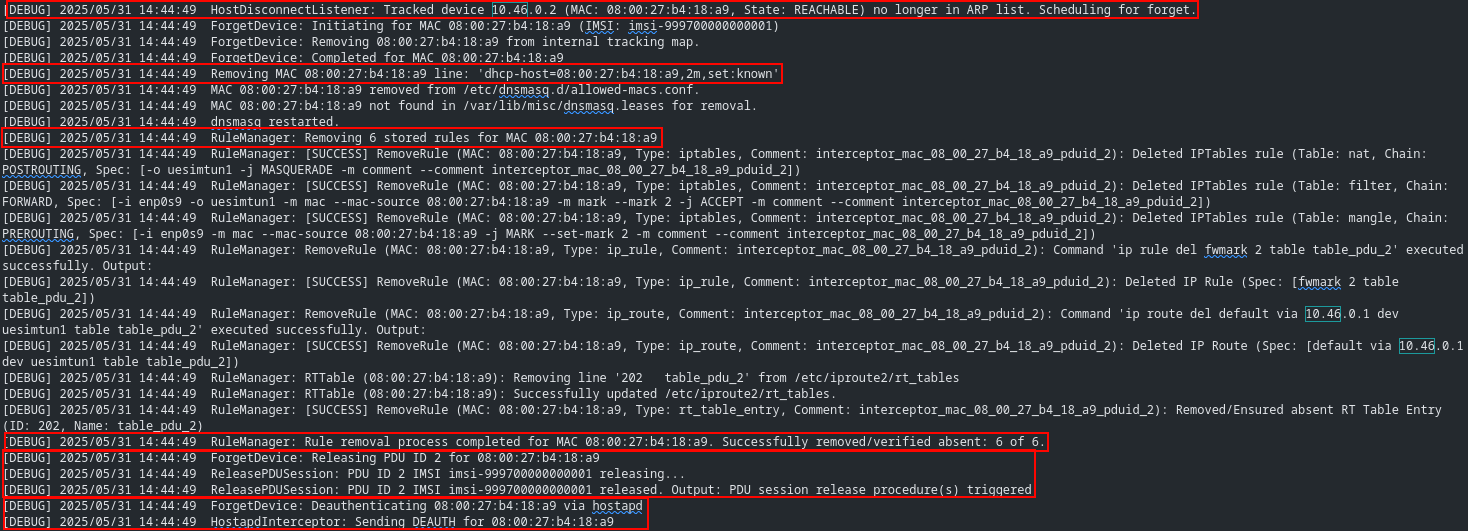
\includegraphics[width=1\linewidth]{figs/naun3_removed.png}
    \caption{\texttt{naun301} disconnected and \ac{5G-RG}'s \texttt{interceptor} proceeds to deauthenticating it, removing traffic mapping rules for it, and releasing it's dedicated \ac{PDU} session.}
    \label{fig:naun3_removed}
\end{figure}

\begin{itemize}
    \item \texttt{interceptor} (around 14:44:49 \ac{UTC}) logs, according to Figure \ref{fig:naun3_removed}: \textttt{"Tracked device 10.46.0.2 (MAC: 08:00:27:b4:18:a9, State: REACHABLE) no longer in ARP list. Scheduling for forget."} This is followed by logs indicating removal from \texttt{allowedDevices}, deauthentication via \texttt{hostapd}, removal of \texttt{iptables} rules, and \ac{PDU} session release for \ac{PDU} ID 2.

    \begin{figure}
        \centering
        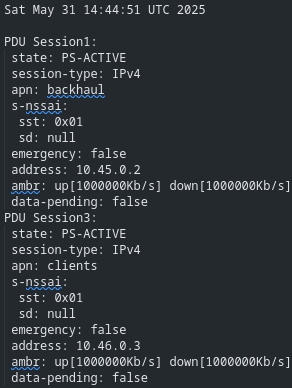
\includegraphics[width=0.20\linewidth]{figs/nr-cli_ps-list.png}
        \caption{\ac{PDU} session listing from UERANSIM}
        \label{fig:nr-cli_ps-list}
    \end{figure}

    \item According to Figure \ref{fig:nr-cli_ps-list}, at 14:44:51 \ac{UTC}, \ac{PDU} Session2 (\ac{IP} \texttt{10.46.0.2}) is no longer listed, while \ac{PDU} Session1 (\texttt{backhaul}) and \ac{PDU} Session3 (for \texttt{naun302}, \ac{IP} \texttt{10.46.0.3}) remain active.

    \begin{figure}
        \centering
        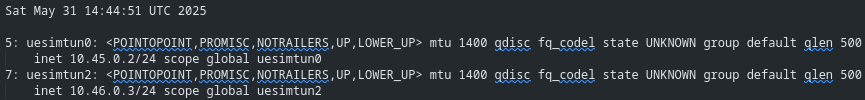
\includegraphics[width=1\linewidth]{figs/ue_pdu_sessions_nics_release.png}
        \caption{\ac{PDU} binded network interfaces after \texttt{uesimtun1} removal}
        \label{fig:ue_pdu_sessions_nics_release}
    \end{figure}
    
    \item Figure \ref{figs:ue_pdu_sessions_nics_release} also confirms that by 14:44:51 \ac{UTC}, the \texttt{uesimtun1} interface (associated with \texttt{10.46.0.2}) is gone, while \texttt{uesimtun0} and \texttt{uesimtun2} persist.

    \begin{figure}
        \centering
        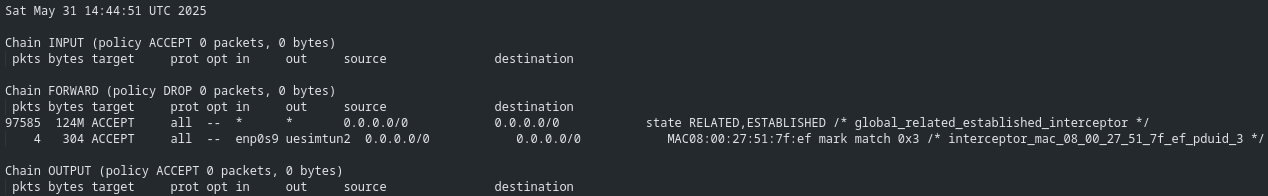
\includegraphics[width=1\linewidth]{figs/ue_naun3_to_pdu_mapping_rules.png}
        \caption{Mapping rules after \texttt{naun301} disconnect and \ac{PDU} Session2 release}
        \label{fig:ue_naun3_to_pdu_mapping_rules}
    \end{figure}

    \item Lastly, Figure \ref{figs:ue_naun3_to_pdu_mapping_rules} also hows that at 14:44:51 \ac{UTC}, the \texttt{iptables} \texttt{FORWARD} rule for \ac{MAC} \texttt{08:00:27:b4:18:a9} (\ac{PDU} ID 2) has been removed, while the rule for \ac{MAC} \texttt{08:00:27:51:7f:ef} (\ac{PDU} ID 3) remains.
\end{itemize}

These results collectively demonstrate that the proposed mechanisms for \ac{NAUN3} device authentication, proxy identity creation via dedicated \ac{PDU} sessions, per-device traffic mapping and \ac{NAT}, and lifecycle management function correctly within the simulated environment.

\section{Security Evaluation}

The security aspects of the solution were evaluated qualitatively based on the implemented mechanisms and observations from the test scenarios.

\begin{itemize}
    \item \textbf{\ac{EAP-TLS} Authentication Integrity:} The logs from \texttt{wpa\_supplicant} in the \acs{NAUN3}, \texttt{hostapd}, and FreeRADIUS consistently show the successful completion of the \ac{EAP-TLS} handshake. This includes the exchange of certificates and the mutual verification steps inherent to the protocol. For instance, FreeRADIUS logs details like \texttt{"eap\_tls: (TLS) Connection Established"} and \texttt{"eap: Sending EAP Success"}. This provides confidence that the local authentication of \ac{NAUN3} devices is cryptographically secured as per \ac{EAP-TLS} standards.

    \item{
        \textbf{Traffic Segregation (Control vs. User Plane):}
        \begin{itemize}
            \item In Figure \ref{fig:RADIUS_traffic_via_backhaul} a Wireshark capture clearly shows \ac{RADIUS} packets (\ac{UDP} port 1812), which carry the \ac{EAP} authentication messages, being exchanged between the \ac{5G-RG}'s \texttt{backhaul} \ac{PDU} session \ac{IP} (\texttt{10.45.0.2}) and the FreeRADIUS server's \ac{IP} (\texttt{10.45.0.1}). This confirms that sensitive authentication control plane traffic is isolated to the dedicated \texttt{backhaul} \ac{DNN}.

            \begin{figure}
                \centering
                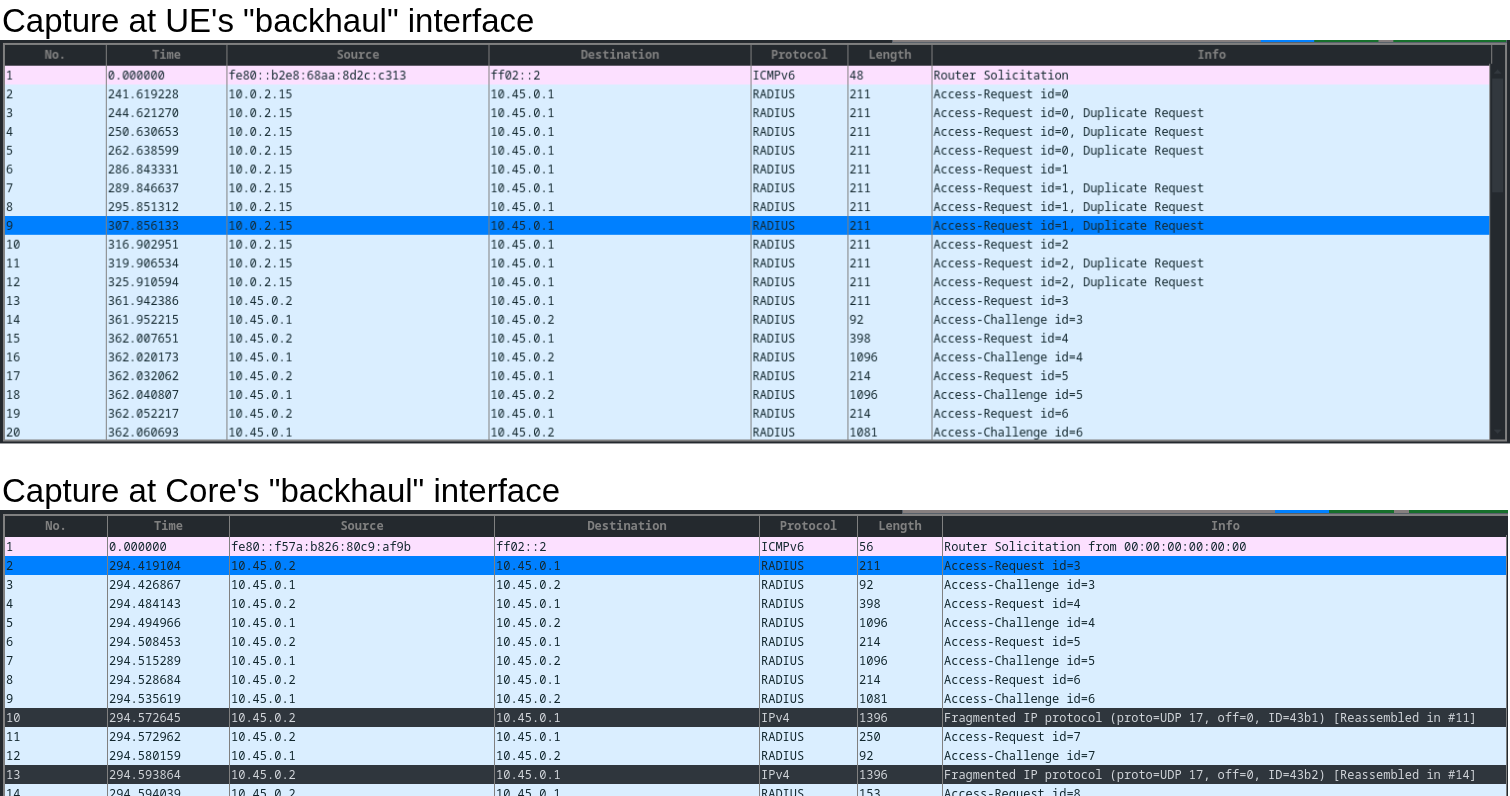
\includegraphics[width=0.75\linewidth]{figs/RADIUS_traffic_via_backhaul.png}
                \caption{\ac{RADIUS} traffic captured at \texttt{backhaul} channel via Wireshark}
                \label{fig:RADIUS_traffic_via_backhaul}
            \end{figure}

            \item The \texttt{hostapd} log (see Listing \ref{lst:hostapd_fail} ) further details the \ac{RADIUS} exchange, initially attempting to send from a default system \ac{IP} (e.g., \texttt{10.0.2.15}) and failing (evident by retransmissions), then succeeding once the \texttt{own\_ip\_addr} (\texttt{10.45.0.2} - the \texttt{backhaul} \ac{PDU} session \ac{IP}) is correctly used. This highlights the correct binding and use of the \texttt{backhaul} \ac{PDU} for \ac{RADIUS}.

\begin{lstlisting}[caption=hostapd failing due to wrong local address,label={lst:hostapd_fail}]
(...)
25 | 1748702388.755637: RADIUS local address: 10.0.2.15:42579
(...)
216| 1748702566.372520: RADIUS local address: 10.45.0.2:50371
(...)
\end{lstlisting}

            \item Conversely, user plane traffic from \ac{NAUN3} devices (e.g., \texttt{iperf3} data in Figure \ref{fig:iperf_naun3_to_core} and ping traffic in Figure \ref{fig:ping_gw}) is shown to originate from the \texttt{clients} \ac{DNN} \ac{IP} addresses (e.g., \texttt{10.46.0.2}, \texttt{10.46.0.3}) assigned to their respective \ac{PDU} sessions. This demonstrates effective segregation between the authentication control plane and the user data plane.
        \end{itemize}
    }
\end{itemize}

While these observations do not constitute a formal penetration test or vulnerability assessment, they confirm that the fundamental security design principles, strong local authentication via \ac{EAP-TLS}, segregation of control and user plane traffic via distinct \acp{DNN}, and abstraction of local \ac{NAUN3} device identities from the \ac{5GC}, are correctly implemented and operational within the test environment. The envisioned enhancement suggests a pathway to more integrated policy control if desired in future iterations.

\section{Performance Evaluation}

% Present the results related to the performance metrics defined earlier (e.g., authentication delay, computational overhead on involved network functions).

% Compare these results against baseline scenarios or standard procedures if possible.

\section{Discussion and Analysis}

The validation results presented in the preceding sections provide substantial evidence for the functional viability and integrity of the proposed framework for integrating Wi-Fi-only/\ac{NAUN3} devices into a \ac{5G} network. This discussion will interpret these findings in the context of the initial research objectives and requirements, compare the solution with standard \ac{3GPP} approaches, and acknowledge observed limitations.

\subsection{Interpretation of Results and Effectiveness in Meeting Requirements}

The primary goal was to devise a solution that allows \ac{NAUN3} devices, which lack \ac{5G} credentials, to securely access \ac{5G} network services with minimal impact on the devices themselves and the standard \ac{5GC}.

\begin{itemize}
    \item \textbf{Local Authentication (Requirement Met):} The successful \ac{EAP-TLS} authentication demonstrates that \ac{NAUN3} devices can be securely authenticated at the edge by the \ac{5G-RG} before any \ac{5G} resources are committed. This meets the requirement for a robust local authentication mechanism.

    \item \textbf{Individual Device Handling and Proxy Identity (Requirement Met):} The core concept of using a dedicated \ac{PDU} session as a proxy identity for each \ac{NAUN3} device was successfully implemented and validated. The \ac{UE} logs and Figures \ref{fig:ue_pdu_sessions_nics} and \ref{fig:iptable_mapping_rules} clearly show the dynamic creation of distinct \ac{PDU} sessions on the \texttt{clients} \ac{DNN}, each with a unique \ac{5GC}-assigned \ac{IP} address, corresponding to each authenticated \ac{NAUN3} device. The \texttt{interceptor} logs (see Figure \ref{fig:interceptor_eap_success}) further detail the interceptor application's role in orchestrating these \ac{PDU} session establishments via \texttt{nr-cli} upon \ac{EAP} success.

    \item \textbf{Traffic Mapping and Isolation (Requirement Met):} The \texttt{ping -R} tests (Figure \ref{fig:ping_gw}) and \texttt{iperf3} results (Figure \ref{fig:iperf_naun3_to_core} showing distinct source \acp{IP} \texttt{10.46.0.2} and \texttt{10.46.0.3}) confirm that traffic from each \ac{NAUN3} device is correctly \textit{NATted} and routed through its unique \ac{PDU} session. The Wireshark capture in Figure \ref{fig:naun3_to_core_ue_view} and the dynamic \texttt{iptables} rules in Figure \ref{fig:iptable_mapping_rules} further substantiate that the \ac{5G-RG} effectively maps local device traffic to its designated \ac{5G} \ac{PDU} session, ensuring traffic isolation.

    \item \textbf{Minimal Core Network and Device Impact (Requirement Met):} The solution operates without requiring any modifications to the \ac{NAUN3} devices beyond standard \ac{EAP-TLS} supplicant capabilities. The \ac{5GC} (Open5GS) interacts with the \ac{5G-RG} as a standard \ac{UE} requesting \ac{PDU} sessions; no changes to core \acp{NF} were needed beyond configuration (\acp{DNN}, subscriber data for the \ac{5G-RG}). This fulfills the critical requirement of minimal disruption.

    \item \textbf{Gateway-Centric Logic (Requirement Met):} All the specialized logic for \ac{NAUN3} authentication relay, \ac{PDU} session orchestration, and traffic mapping is concentrated within the \ac{5G-RG} (\texttt{ue} \ac{VM}), primarily within the custom \texttt{interceptor} application and configurations of \textt{hostapd} and \texttt{dnsmasq}.

    \item \textbf{Lifecycle Management (Requirement Met):} The logs in Figures \ref{fig:naun3_removed}, \ref{fig:ue_pdu_sessions_nics_release} and \ref{fig:ue_naun3_to_pdu_mapping_rules} demonstrate that upon simulated \ac{NAUN3} device disconnection, the \texttt{interceptor} correctly triggers local deauthentication, \ac{PDU} session termination, and cleanup of associated routing rules and \ac{DHCP} permissions.

    \item \textbf{Traffic Segregation (Requirement Met):} The capture seen in Figure \ref{fig:RADIUS_traffic_via_backhaul} confirm that authentication control plane traffic (\ac{RADIUS}/\ac{EAP}) is successfully segregated onto the \texttt{backhaul} \ac{DNN}, using the \ac{5G-RG}'s \ac{PDU} session \ac{IP} designated for this purpose, while \ac{NAUN3} user plane traffic utilizes the separate \texttt{clients} \ac{DNN} \ac{PDU} sessions.
\end{itemize}